%Version 3.1 December 2024
% See section 11 of the User Manual for version history
%
%%%%%%%%%%%%%%%%%%%%%%%%%%%%%%%%%%%%%%%%%%%%%%%%%%%%%%%%%%%%%%%%%%%%%%
%%                                                                 %%
%% Please do not use \input{...} to include other tex files.       %%
%% Submit your LaTeX manuscript as one .tex document.              %%
%%                                                                 %%
%% All additional figures and files should be attached             %%
%% separately and not embedded in the \TeX\ document itself.       %%
%%                                                                 %%
%%%%%%%%%%%%%%%%%%%%%%%%%%%%%%%%%%%%%%%%%%%%%%%%%%%%%%%%%%%%%%%%%%%%%

%%\documentclass[referee,sn-basic]{sn-jnl}% referee option is meant for double line spacing

%%=======================================================%%
%% to print line numbers in the margin use lineno option %%
%%=======================================================%%

%%\documentclass[lineno,pdflatex,sn-basic]{sn-jnl}% Basic Springer Nature Reference Style/Chemistry Reference Style

%%=========================================================================================%%
%% the documentclass is set to pdflatex as default. You can delete it if not appropriate.  %%
%%=========================================================================================%%

%%\documentclass[sn-basic]{sn-jnl}% Basic Springer Nature Reference Style/Chemistry Reference Style

%%Note: the following reference styles support Namedate and Numbered referencing. By default the style follows the most common style. To switch between the options you can add or remove “Numbered” in the optional parenthesis. 
%%The option is available for: sn-basic.bst, sn-chicago.bst%  
 
%%\documentclass[pdflatex,sn-nature]{sn-jnl}% Style for submissions to Nature Portfolio journals
%%\documentclass[pdflatex,sn-basic]{sn-jnl}% Basic Springer Nature Reference Style/Chemistry Reference Style
\documentclass[pdflatex,sn-mathphys-num]{sn-jnl}% Math and Physical Sciences Numbered Reference Style
%%\documentclass[pdflatex,sn-mathphys-ay]{sn-jnl}% Math and Physical Sciences Author Year Reference Style
%%\documentclass[pdflatex,sn-aps]{sn-jnl}% American Physical Society (APS) Reference Style
%%\documentclass[pdflatex,sn-vancouver-num]{sn-jnl}% Vancouver Numbered Reference Style
%%\documentclass[pdflatex,sn-vancouver-ay]{sn-jnl}% Vancouver Author Year Reference Style
%%\documentclass[pdflatex,sn-apa]{sn-jnl}% APA Reference Style
%%\documentclass[pdflatex,sn-chicago]{sn-jnl}% Chicago-based Humanities Reference Style

%%%% Standard Packages
%%<additional latex packages if required can be included here>

\usepackage{graphicx}%
\usepackage{multirow}%
\usepackage{amsmath,amssymb,amsfonts}%
\usepackage{amsthm}%
\usepackage{mathrsfs}%
\usepackage[title]{appendix}%
\usepackage{xcolor}%
\usepackage{textcomp}%
\usepackage{manyfoot}%
\usepackage{booktabs}%
\usepackage{algorithm}%
\usepackage{algorithmicx}%
\usepackage{algpseudocode}%
\usepackage{listings}%
%%%%

%%%%%=============================================================================%%%%
%%%%  Remarks: This template is provided to aid authors with the preparation
%%%%  of original research articles intended for submission to journals published 
%%%%  by Springer Nature. The guidance has been prepared in partnership with 
%%%%  production teams to conform to Springer Nature technical requirements. 
%%%%  Editorial and presentation requirements differ among journal portfolios and 
%%%%  research disciplines. You may find sections in this template are irrelevant 
%%%%  to your work and are empowered to omit any such section if allowed by the 
%%%%  journal you intend to submit to. The submission guidelines and policies 
%%%%  of the journal take precedence. A detailed User Manual is available in the 
%%%%  template package for technical guidance.
%%%%%=============================================================================%%%%

%% as per the requirement new theorem styles can be included as shown below
\theoremstyle{thmstyleone}%
\newtheorem{theorem}{Theorem}%  meant for continuous numbers
%%\newtheorem{theorem}{Theorem}[section]% meant for sectionwise numbers
%% optional argument [theorem] produces theorem numbering sequence instead of independent numbers for Proposition
\newtheorem{proposition}[theorem]{Proposition}% 
%%\newtheorem{proposition}{Proposition}% to get separate numbers for theorem and proposition etc.

\theoremstyle{thmstyletwo}%
\newtheorem{example}{Example}%
\newtheorem{remark}{Remark}%

\theoremstyle{thmstylethree}%
\newtheorem{definition}{Definition}%

\raggedbottom
%%\unnumbered% uncomment this for unnumbered level heads


% ADDED BY THE AUTHORS
\newcommand{\david}[1]{{\small{\color{blue} \sf $\heartsuit$ [David: #1]}}}
\newcommand{\paul}[1]{{\small{\color{green} \sf $\spadesuit$ Paul: #1}}}



\begin{document}

\title[e-values for multiverse analysis]{e-values for multiplicity control in multiverse analysis}

%%=============================================================%%
%% GivenName	-> \fnm{Joergen W.}
%% Particle	-> \spfx{van der} -> surname prefix
%% FamilyName	-> \sur{Ploeg}
%% Suffix	-> \sfx{IV}
%% \author*[1,2]{\fnm{Joergen W.} \spfx{van der} \sur{Ploeg} 
%%  \sfx{IV}}\email{iauthor@gmail.com}
%%=============================================================%%

\author[1]{\fnm{Paul} \sur{Rognon-Vael}}\email{paul.rognon@gmail.com}

\author*[2,3]{\fnm{David} \sur{Rossell}}\email{david.rossell@upf.edu}
%\equalcont{These authors contributed equally to this work.}

\affil*[1]{\orgdiv{Department of Economics and Business}, \orgname{Bocconi University}, \orgaddress{\street{Via Roberto Sarfatti, 25}, \city{Milano}, \postcode{20136}, \country{Italy}}}

\affil*[2]{\orgdiv{Department of Economics and Business}, \orgname{Universitat Pompeu Fabra}, \orgaddress{\street{Ram\'on Trias Fargas 25}, \city{Barcelona}, \postcode{08005}, \country{Spain}}}

\affil[3]{\orgdiv{Data Science Center}, \orgname{Barcelona School of Economics}, \orgaddress{\street{Ram\'on Trias Fargas 25}, \city{Barcelona}, \postcode{08005}, \country{Spain}}}


\abstract{Multiverse analysis refers to a common situation in the Social Sciences where one wishes to assess the association between multiple possible treatment definitions and multiple possible outcome definitions, potentially within multiple sub-populations. Multiverse analysis is particularly useful as an exploratory tool to assess sensitivity to the chosen analysis specification, but it is sometimes also used to assess statistical significance. In the latter case, it is critical to acknowledge that multiple comparisons are being performed, and to ensure a valid statistical control of false positive findings. 
We study the use of e-values within generalized linear models as a tool to control the false discovery rate regardless of the dependence structure of the multiple tests being performed, while accounting for the effect of confounding covariates. 
We compare the performance of several approaches: universal e-values, soft-rank e-values, and p-to-e calibration methods. We find that, for problem characteristics typically encountered in multiverse analyses, p-to-e calibration significantly outperforms the other two approaches in terms of statistical power, but said power may be moderate unless the sample size or effect sizes are large enough. 
An application to a dataset studying the association between technology use on well-being reveals association between depression, low self-steem and peer problems with internet and social media usage.}

\keywords{multiverse analysis, e-value, multiple testing, false discovery rate}

%%\pacs[JEL Classification]{D8, H51}

%%\pacs[MSC Classification]{35A01, 65L10, 65L12, 65L20, 65L70}

\maketitle

\section{Introduction}
\label{sec:intro}


There are many applications where one wants to assess the effect of multiple treatments on multiple outcomes, potentially also separately within multiple sub-populations.
A prominent example in the Social Sciences occurs when one has multiple outcomes that can be conceivably thought of as measuring related underlying characteristics, such as different measures of psychological well-being, several measures of economic activity, or several measures of radicalization in social media usage.
Similarly, the multiple treatments may refer to using various types of technology, realizing various economic interventions, or exposure to various social media unradicalization campaigns.
It may also be natural to wish to assess treatment effects within sub-populations, for example defined by sex and age groups, economic regions, or social media user backgrounds.
Beyond the Social Sciences, similar situations arise in other fields. In Biomedicine one may study the effect of non-identical, but related, treatments on multiple measures of disease progression, in Climate Science one may study the association between multiple human-driven processes on multiple physical parameters, etc.

Multiverse analysis provides a data analysis framework that considers such multiple outcome-treatment-subpopulation combinations.
A key pitfall that it seeks to avoid is selective reporting, whereby researchers obtain treatment effect estimates for all combinations and report only those that are larger or more statistically significant. Critically, selective reporting occurs when a researcher fails to indicate all the outcome-treatment-subpopulation that were considered.
By acknowledging all such combinations, multiverse analysis serves as an excellent tool as an exploratory data analysis method that assesses the sensitivy of results across various analysis specifications.
In some instances, researchers may be interested in going beyond a descriptive analysis to also report some assessment of statistical significance. In such circumstances one may wish to control some measure of false discoveries, and it is then critical to account for the multiple comparisons when assessing the statistical significance of the findings. This is the strategy followed in this paper.

Before proceeding, we discuss another popular strategy: focus the analysis on some summary measure across all the comparisons being made. 
This is the standard approach for meta-analyses in the medical literature, where one combines the evidence regarding the effect of a medical treatment (or family or related treatments) across studies (typically, randomized clinical trials). Therein, it is common to account for treatment effect heterogeneity, often driven by differences in the patient population targeted by each study.
A notable example in the Social Sciences, where randomized trials are rare, is Specification Curve Analysis (SCA, \cite{simonsohn:2020}). By default, SCA reports the median estimated effect across treatment-outcome-subpopulations, and assesses the statistical significance of this single parameter.
An advantage of using a single summary measure over multiple comparison adjustments is that, since no significance corrections are needed, if all treatment effects are comparable then one may have higher statistical power to detect that the summarized effect truly exists.
However, we urge strong caution in the sense that aggregate measures should only be used in appropriate circumstances.
A critical pitfall is that, when the treatments are not comparable or there is significant heterogeneity in their effects, the aggregate measure may be highly misleading.
For example, \cite{semken:2022} showed that SCA led \cite{orben:2019} to erroneously conclude that the association between technology use and teenager well-being was practically negligible. The reason was that the association was near-zero for some technologies such as television use, but large for others such as mobile phone use, and hence overall mild on the average.
Another critical issue arises when the aggregate measure is obtained across multiple possible subsets of control covariates, an option that is explicitly considered in SCA.
This is inadequate because one combines quantities that have a different statistical meaning, such as marginal and conditional associations, and hence the summary has no natural interpretation. % (on top of heterogeneity issues mentioned earlier, which may also occur across subsets of control covariates).
For example, assessing the conditional association between salary and gender given an individual job's position, education and other characteristics has a different meaning than assessing the marginal association between salary and gender. Namely, a marginal association between gender and salary can be partially driven by people from different genders making different career choices, whereas an association between gender and salary within people with the same job position, education and characteristics suggests salary discrimination. %\paul{I think "gender" would be more appropriate than sex} \david{In a previous paper a referee complained that we used gender, and said that sex was more appropriate. To be precise, both are reasonable, sex is based on biology and gender on self-identification, and the example that we mention can be applied to either. So take your pick, I'm happy either way. :-)} \paul{I think that in this case discrimination would be based on gender, to be precise not even self-identified gender but perceived gender, rather than biological sex. There is a bit of politics around the sex/gender wording but given the journal we will be submitting (Journal of Sociological Methods and Research), my bet would be that "gender" is preferred by reviewers.}
See \cite{semken:2022} for an in-depth discussion of issues with SCA.

In this paper we study the use of a simple and practical approach to multiplicity control in multiverse analysis based on e-values. %The approach is discussed by \cite{ramdas:2025} (Chapter 5.2), and combines ideas from likelihood ratio tests and Bayes factors.
Briefly, e-values are an increasingly popular framework for hypothesis testing that has several features relative to p-values. %\paul{should we write "p-value" since we write "e-value"?}
When comparing two hypotheses, e-values accumulate evidence against the null hypothesis similarly to a Bayes factor (see \cite{kass_raftery:1995} for a review). Further, e-values guarantee a strict control of the type I error probability, and are particularly suited to control the false discovery rate (FDR) in multiple comparisons \citep{wang_ruodu:2022}. Although less relevant to this work, e-values also enable anytime-valid inference, a strong asset in settings where one accumulates data and makes decisions sequentially. %Universal inference e-values are a type of e-value which (as the name suggests) can be applied to any setting, including those where test statistics follow an unknown distribution and hence p-values are not applicable.
For seminal papers on e-values see \cite{vovk:2021,gruenwald:2024,chugg:2026}, and for an excellent monograph see \cite{ramdas:2025}.

We briefly review the rich literature on FDR control for multiple testing.
\cite{benjamini:1995} proposed that, when conducting many statistical tests, one should use procedures that guarantee controlling the FDR below a user pre-specified level $\alpha$. The FDR is the expected proportion of false positives among the hypotheses that are claimed as statistically significant.
\cite{benjamini:1995} proposed a p-value adjustment procedure that controls the FDR under the assumption that the tests are independent, and \cite{benjamini:2001} a variation that assumes that the tests follow a type of positive dependence structure.
A large body of subsequent work extended the FDR framework in several directions.
A prominent example are the q-values of~\cite{storey:2003}.
Analogously to p-values controlling the expected number of false discoveries, q-values control the expected positive FDR, that is the expected fraction of false discoveries, conditional on $\geq 1$ discoveries being reported.
% which estimates the FDR associated with each individual hypothesis using an estimate of the proportion of true null hypotheses.
However, q-values require estimating nuisance parameters such as the proportion of true null hypotheses, and therefore do not control the FDR exactly. Further, estimating said nuisance parameters often requires simplifying assumptions such as independence between the test statistics, which rarely hold in practice.
Another influential line of work is based on the local FDR~\citep{efron:2001}, which is embedded into an empirical Bayes framework. The local FDR can be interpreted as the posterior probability that a given hypothesis is null, given the value of the test statistic for that hypothesis. The local FDR provides a more refined, hypothesis-specific, assessment of significance than tail-area measures such as q-values. 
Estimating the local FDR accurately requires the number of hypotheses being tested to be large (at least in the hundreds), assuming independence across tests, and making certain choices when estimating the global mixture distribution of the test statistics.
Further related work includes the optimal discovery procedure of~\cite{storey:2007}, and the Bayesian discovery procedure of~\cite{guindani:2009}. See~\cite{efron:2012} for a monograph on FDR control.

An advantage of e-values over these methods are that they provide a finite-$n$ FDR control that does not require estimating nuisance parameters, and which holds regardless of the dependence structure between the multiple tests. This is relevant in multiverse analysis, where typically tests cannot be assumed independent.
Another advantage of e-values for multiverse analysis is that they are more composable, for example they can be multiplied or averaged across independent datasets (corresponding to subpopulations where a treatment effect is tested, for example) to obtain valid e-values.
A main limitation of e-values relative to methods based on p-values, q-values and empirical Bayes is that the latter usually have a higher statistical power, provided that their assumptions hold. 
Therefore, e-values are most appropriate for datasets where one has relatively large sample sizes. Otherwise, while FDR control is ensured, one may obtain few statistically significant findings. In this paper, we consider several strategies to obtain e-values and compare their power via simulation studies that mimic common sample sizes and problem dimensions encountered in multiverse analysis within the Social Sciences. Our findings suggest that simple p-to-e calibration rules, which convert a p-value into an e-value, attain higher statistical power than generic strategies such as universal e-values \citep{wasserman:2020} and soft-rank e-values \citep{koning:2024}. 


The paper is structured as follows. In Section~\ref{sec:framework} we introduce notation and lay out a generalized linear model framework for treatment effect estimation within the context of a multiverse analysis.
Section~\ref{sec:evalues} reviews e-values, discusses issues related to statistical power and their use for multiplicity control.
Section~\ref{sec:results} applies our methodology to a dataset studying the association between teenager mental well-being and technology use.
Section~\ref{sec:discussion} concludes.


\section{Framework}
\label{sec:framework}


We lay out a multiverse framework that is based on generalized linear models and closely resembles that of \cite{semken:2022} but provides FDR control guarantees through e-values.
Consider a setting where one has $L$ outcomes, $p_x$ treatments and $p_z$ control covariates, with $n$ observations for each.
Said observations may be potentially split across $p_g \geq 1$ subpopulations.
Let $y^{(l)} \in \mathbb{R}^n$ for $l=1,\ldots,L$ be the observed outcomes,
$X$ the $n \times p_x$ matrix and $Z$ the $n \times p_z$ with the treatment and control covariates (respectively),
and $G$ a $n \times p_g$ matrix enconding the subgroup information (if one is not interested in subgroups, then $G$ is omitted).
Let $x_i$, $z_i$ and $g_i$ be the $i^{th}$ row in $X$, $Z$ and $G$ respectively.
Throughout, we denote expectations by $\mathbb E$, probabilities by $\mathbb P$, and by $\mathbb E_P$ and $\mathbb P_P$ expectations and probabilities when data are generated by a specific distribution $P$.
Further, we denote by $p$ the density (or probability mass) function associated to a distribution $P$, and by $q$ those associated to a distribution $Q$.

A generalized linear model for outcome $l$ assumes that
\begin{align}
  F( \mathbb E (y_i^{(l)} \mid x_i, z_i, g_i) )=
  \beta_0^{(l)} + z_i^T \eta_z^{(l)} + g_i^T \eta_g^{(l)} + \sum_{j=1}^{p_x} (\beta_j^{(l)} + g_i^T \delta_j^{(l)}) x_{ij},
\label{eq:outcome_equation}
\end{align}
where $F$ is the link function (e.g., the identity for linear regression, or the logit for logistic regression),
$\beta_0^{(l)} \in \mathbb{R}$ is the intercept,
$\beta_j^{(l)} \in \mathbb{R}$ the average effect of treatment $j$ on outcome $l$,
$\delta_j^{(l)}$ captures subpopulation-specific effects,
and $\eta_z^{(l)} \in \mathbb{R}^{p_z}$ and $\eta_g^{(l)} \in \mathbb{R}^{p_g}$ are coefficients associated to control covariates and subgroups respectively.
We denote the whole parameter vector by $\theta^{(l)}= (\{ \beta_j^{(l)} \}_{j=0}^{p_x}, \{ \delta_j^{(l)} \}_{j=1}^{p_x}, \eta_z^{(l)}, \eta_g^{(l)})$.
Importantly, to be able to interpret $\beta_j^{(l)}$ as an average treatment effect, $g_i \in \mathbb{R}^{p_g}$ must encode subpopulation information using a specific weighted sum-to-zero constraint described next.
Let $\rho_k$ be the proportion of observations coming from subpopulation $k$, we define
\begin{align}
  g_{ik}= \begin{cases}
    \rho_k  \mbox{, if observation } i \mbox{ comes from subpopulation } k \\
    - (1 - \rho_k) \mbox{, otherwise}
    \end{cases}
\nonumber
\end{align}
for $k=1,\ldots,p_g$, which implies that $\sum_{i=1}^n g_{ik}=0$.
We define the effect of treatment $j$ on outcome $l$ for individual $i$ in subpopulation $k$ as
\begin{align}
\beta_{jk}^{(l)}=  \frac{\partial}{\partial x_{ij}} F(\mathbb E (y_i^{(l)} \mid x_i, z_i, g_i)) 
= \beta_j^{(l)} + g_i^T \delta_j^{(l)}
= \beta_j^{(l)} + \rho_k \delta_{jk}^{(l)} - \sum_{m \neq k} \delta_{jm}^{(l)} (1 - \rho_m).
\nonumber
\end{align}
The corresponding average treatment effect (ATE) across all individuals is
\begin{align}
\frac{1}{n} \sum_{i=1}^n \frac{\partial}{\partial x_{ij}} F(\mathbb E (y_i^{(l)} \mid x_i, z_i, g_i))
= \beta_j^{(l)} + \frac{1}{n} \left( \sum_{i=1}^n g_i^T \right) \delta_j^{(l)}= \beta_j^{(l)}.
\nonumber
\end{align}

We consider a multiverse analysis where one is interested in estimating the ATEs $\beta_j^{(l)}$ for $l=1,\ldots,L$ and $j=1,\ldots,p_x$,
and performing the corresponding $L p_x$ hypothesis tests
\begin{align}\label{eq:test}
H_{lj}: &\beta_j^{(l)}= 0, \beta_{j'}^{(l)} \neq 0 \mbox{ for } j' \neq j
\nonumber
\\
\overline{H}_l: & \beta_{j'}^{(l)} \neq 0 \mbox{ for } j' \in \{1,\ldots,p_x\}
\end{align}
That is, the null hypothesis $H_{lj}$ is that treatment $j$ has zero effect on outcome $j$, without any restrictions on the remaining treatment effects.
And there is a global alternative hypothesis $\overline{H}_l$, shared across all treatments, that all treatment effects are non-zero.
We denote by $\mathcal{H}_{lj}$ the set of probability distributions such that $H_{lj}$ holds, and by $\overline{\mathcal{H}}_l$ the set where none of $\overline{H}_l$ holds.
In the event that one is also interested in testing the effect within subpopulations, there are $L p_x p_g$ further tests corresponding to $H_{ljk}: \beta_{jk}^{(l)}=0$ for  $l=1,\ldots,L$, $j=1,\ldots,p$ and $k=1,\ldots,p_g$.
To ease notation we drop the subscript $k$ in the exposition below, that is we describe the case where there are no subpopulations, but our framework remains readily applicable when sub-populations are also of interest.

Although not stated explicitly, none of the remaining parameters in $\theta^{(l)}$ are assumed to be zero, neither under the null nor the alternative.
In particular, the control covariates effects $\eta_z$ are always assumed to be non-zero.
This is contrast to SCA \citep{simonsohn:2020} or its Bayesian counterpart \citep{semken:2022}, where one also considers covariate subsets.
As discussed in Section~\ref{sec:intro}, SCA computes a median over subsets of control covariates that has no statistical interpretation. Its Bayesian counterpart computes a weighted average where weights are given by posterior model probabilities, which as $n \to \infty$ converges to performing inference under a model that includes only the controls that have non-zero effects.
While this implies an asymptotic gain in statistical power, one does not obtain strict type I error control for finite $n$.
Hence our strategy here of including all controls, as an alternative that is more conservative but strictly controls false positives.


Given the potentially large number of multiple tests being conducted, it is important to assess statistical significance in a way such that some measure of false positives is controlled.
Specifically, we consider the FDR \citep{benjamini:1995}. Let $\gamma_{lj}= \mbox{I}(\beta_j^{(l)} \neq 0)$ be the indicator that the null hypothesis $H_{lj}$ does not hold, let $\hat{\gamma}_{lj} = 1$ if we reject $H_{lj}$ and $\hat{\gamma}_{lj}=0$ otherwise. 
Then the number of false positive is $\sum_{l,j} \gamma_{lj} \hat{\gamma}_{lj}$, the number of rejected null hypotheses is $\sum_{l,j} \hat{\gamma}_{lj}$, and $\mbox{FDR}= \mathbb E(\mbox{FDP})$, where 
\begin{align}
 \mbox{FDP}= \begin{cases}
\frac{\sum_{l,j} \gamma_{lj} \hat{\gamma}_{lj}}{\sum_{l,j} \hat{\gamma}_{lj}} \mbox{, if } \sum_{l,j} \hat{\gamma}_{lj} > 0
\nonumber \\
0  \mbox{, otherwise} 
\end{cases}
\nonumber
\end{align}
and the expectation is with respect to the data-generating distribution.
That is, the FDR is the expected false discovery proportion (FDP) and, if no hypotheses are rejected, then FDP is defined to be 0.
If one is interested in testing subpopulation effects $\beta_{jk}^{(l)}$, then the FDR is analogously defined by taking sums over $k$ as well.



\section{e-values}
\label{sec:evalues}

E-values provide a framework to assess statistical significance that conveniently allows the FDR to be controlled, regardless of the dependence structure between the tests being performed.
Formally, an e-value is the realization of a random variable called an e-variable, whose defining property is that its expectation under the null hypothesis is $\leq 1$.

\begin{definition}
Consider a null hypothesis $H_{lj}$ specifying a set of probability distributions $\mathcal{H}_{lj}$.
A test statistic $E_{lj}$ is an e-variable if and only if
$\mathbb E_P (E_{lj}) \leq 1$ for any $P \in \mathcal{H}_{lj}$.
\label{def:evariable}
\end{definition}

Larger values of $E_{lj}$ provide stronger evidence for the alternative hypothesis.
By Markov's inequality, if one rejects $H_{lj}$ when $E_{lj} \geq 1/\alpha$, then the type I error is $\leq \alpha$:
\begin{align}
 \mathbb P_P \left( E_{lj} \geq \frac{1}{\alpha} \right) \leq \alpha \mathbb E_P(E_{lj}) \leq \alpha,
\nonumber
\end{align}
for any $P \in \mathcal{H}_{lj}$.

In Section~\ref{ssec:define_evariables} we review some strategies to define e-variables. 
In Section~\ref{ssec:simstudy}, we use simulations to assess the statistical power of several such strategies in linear and logistic regression. Section~\ref{ssec:fdr_control} reviews e-value-based procedures for FDR control.


\subsection{Defining e-variables}
\label{ssec:define_evariables}

There are many ways to define valid e-variables. While the Markov inequality guarantees type I error control for all e-variables, their statistical power may vary greatly. Efforts have been made to define e-variables that accumulate evidence against the null as fast as possible. Such optimality is usually defined in terms of maximizing $\mathbb E_Q [\log E_{lj}]$, where $Q \in \overline{\mathcal{H}}_l$ is a distribution within the alternative hypothesis. 
One possible definition of optimality is the so-called numeraire (\cite{ramdas:2025}, Chapter 6), an e-variable $E_{lj}^*$ that is defined by $E_{lj}/E_{lj}^*$ having expectation $\leq 1$ under the alternative, where $E_{lj}$ is any other e-variable. 
Another possible definition by \cite{gruenwald:2024} uses a worst-case optimality criterion called GROW.
When testing a point null hypothesis versus a point null alternative, both definitions return the likelihood-ratio test as the optimal e-variable. This is of course not applicable to our setting, where the null hypothesis $\mathcal{H}_{lj}$ contains infinitely many distributions indexed by $\theta^{(l)}$, and so does the alternative $\overline{\mathcal{H}}_l$.
In such more general settings, obtaining either the numeraire or the GROW-optimal e-variable is related to so-called reverse information projections (RIP), and it is a highly non-trivial task.

We review next some practical alternatives applicable to our generalized linear model framework~\eqref{eq:outcome_equation}:
universal mixture e-variables, soft-rank e-variables and p-to-e calibration.
Universal inference is a framework introduced by \cite{wasserman:2020} %The approach is practical, in that it is easy to implement and can be used in arbitrarily complex settings, the downside being that its power is dominated by that of the numeraire (\cite{ramdas:2025}, Chapter 6.5). 
%The original approach of \cite{wasserman:2020} uses split likelihood-ratio e-variables. 
where one splits the observed data $y^{(l)}=(y_0^{(l)},y_1^{(l)})$, and $y_0^{(l)}$ is assumed independent from $y_1^{(l)}$. One then obtains the maximum likelihood estimate (MLE) for the density function under the null $\hat{p}_{lj} \in \mathcal{H}_{lj}$ using only $y_0^{(l)}$, that under the alternative $\hat{q}_l$ using only $y_1^{(l)}$, and the split likelihood-ratio e-variable proposed in \cite{ramdas:2026} is defined as $E_{lj}= \hat{q}_l(y_0^{(l)}) / \hat{p}_{lj}(y_0^{(l)})$.
Universal mixture e-variables are a variation discussed in \cite{ramdas:2025} (Chapter 5.2) that avoids using arbitrary data splits (as well as assuming independence) by considering a hybrid of frequentist and Bayesian hypothesis tests.
Specifically, let $\hat{p}_{lj} \in \mathcal{H}_{lj}$ be the MLE under the null, now using the full data $y^{(l)}$. Define
\begin{align}
E^{um}_{lj}= \frac{q_l(y^{(l)})}{\hat{p}_{lj}(y^{(l)})},
\label{eq:univ_evalue_mixture}
\end{align}
where
\begin{align}
 q_l(y)= \int p(y \mid \theta^{(l)}) p(\theta_l \mid \overline{H}_l) d\theta_l
\nonumber
\end{align}
is the marginal (or integrated) likelihood with respect to a prior density $p(\theta_j^{(l)} \mid \overline{H}_l)$ that places full support on the alternative %, that is such that $P(y \mid \theta_{lj}) \not\in \mathcal{H}_{lj}$ with prior probability 1  
(i.e., such that the prior probability that $\theta_j^{(l)} \neq 0$ is 1).
It is easy to show that $E_{lj}$ is an e-variable for any choice of $p(\theta_j^{(l)} \mid \overline{H}_l)$.
Since $\hat{p}_{lj}$ is the MLE under $\mathcal{H}_{jl}$, by definition we have that $p(y^{(l)}) \leq \hat{p}_{lj}(y^{(l)})$ for any $P \in \mathcal{H}_{lj}$, therefore
\begin{align}
 \mathbb E_{P} \left( E_{lj} \right)=
\int \frac{q_l(y^{(l)})}{\hat{p}_{lj}(y^{(l)})} p(y^{(l)}) dy^{(l)}
\leq \int \frac{q_l(y^{(l)})}{p(y^{(l)})} p(y^{(l)}) dy^{(l)}= \int q_l(y^{(l)}) dy^{(l)}= 1.
\nonumber
\end{align}
In our framework~\eqref{eq:outcome_equation}, to avoid subjectivity in the choice of $p(\theta_j^{(l)})$, one may consider Zellner's unit information prior \citep{zellner:1986}, a classical default that has tight connections to the Bayesian information criterion \citep{schwarz:1978}.
Specifically, let $W=(X, Z, G)$ be the design matrix associated to the regression equation in~\eqref{eq:outcome_equation} (if subpopulations are of interest, then the interaction terms $GX$ are also included in $W$).
Zellner's unit information prior is
\begin{align}
\theta_j^{(l)} \sim N(0, n \sigma_l^2 (W^T W)^{-1}),
\label{eq:uip}
\end{align}
where $\sigma_l^2 > 0$ is the GLM dispersion parameter associated to $y^{(l)}$.
This choice assumes that $W^T W$ is invertible, as is the case in our examples here, otherwise an alternative default is to replace $W^TW$ by $\mbox{diag}(W^T W)$. Expression~\eqref{eq:univ_evalue_mixture} requires obtaining an MLE for the $L p_x$ alternative hypotheses, which can be done efficiently and in parallel using any suitable optimization algorithm.
It also requires obtaining $L$ marginal likelihoods $q_l(y)$, one for each outcome.
In the linear regression case where $y^{(l)} \sim N(W \theta^{(l)}, \sigma_l^2 I)$, $q_l$ has a closed-form.
Specifically, if one sets an inverse Gamma prior $\sigma_l^2 \sim \mbox{IG}(a/2,l/2)$, then
\begin{align}
 \frac{q_l(y^{(l)})}{\hat{p}_{lj}(y^{(l)})}= 
\frac{l^{a/2} \Gamma(\frac{n+a}{2})}{(n + 1)^{d/2} \Gamma(a/2)}
\frac{(2 e/\hat{\sigma}_l^2)^{\frac{n}{2}}}{\left( l+ \| y^{(l)} \|^2 - \frac{n}{n+1} (\hat{\theta}^{(l)})^T W^T W \hat{\theta}^{(l)} \right)^{\frac{n + a}{2}}}
\nonumber
\end{align}
where $\| \cdot \|^2$ is the squared Euclidean norm, $d=\mbox{dim}(\theta^{(l)})$, $\hat{\theta}^{(l)}= (W^T W)^{-1} W^T y^{(l)}$ is the least-squares estimator and $\hat{\sigma}_l^2= n^{-1}(\| y^{(l)} \|^2 - \| W \hat{\theta}^{(l)} \|^2)$ the MLE for the error variance.
Outside of linear regression numerical integration methods must be used and, as long as the number of outcomes $L$ is not too large, this can also be done quickly (and in parallel).
One may approximate $q_l$ using Laplace approximations, which is very fast as it requires a single optimization exercise for each outcome, and is very accurate as $n$ grows (\cite{kass:1990}, \cite{rossell:2021b} Lemma S3).

A second possible strategy is to use soft-rank e-variables \citep{koning:2024}. 
These are typically based on permutation exercises akin to those used to obtain permutation-based p-values, therefore they are more computationally-intensive but as a positive aspect they are more reliable when our statistical model in \eqref{eq:outcome_equation} is misspecified (e.g., covariate effects are truly non-linear, errors are heteroskedastic, etc.).
Let $T_0$ be a test statistic for the null hypothesis of interest, and let $T_1,\ldots,T_B$ be the realization of $B$ test statistics that are exchangeable with $T_0$ under the null. The soft-rank e-variable is 
\begin{align}
  E^{sr} \,=\,\frac{(B+1)T_0}{\sum_{b=0}^{B}T_b}.
\end{align}
%The assumed exchangeability guarantees that $E^{sr}$ is indeed an e-variable. 
In generalized linear models, %~\eqref{eq:outcome_equation}, 
$T_0$ can be the likelihood ratio associated to \eqref{eq:test},
\begin{equation}\label{eq:lrt}
  T_0=\frac{\hat{q}_l(y^{(l)})}{ \hat{p}_{lj}(y^{(l)})}
\end{equation}
where recall that $\hat{p}_{lj}$ is the MLE for the density function under the null hypothesis $H_{lj}$, and $\hat{q}_l$ that under the alternative. 
Exchangeable likelihood ratio test statistics $T_1,\ldots,T_B$ can be obtained using permutations. 
Let $y^{(l,b)}$ be a permuted version of $y^{(l)}$ such that the null hypothesis $H_{lj}$ holds, and define
\[T_b=\frac{\hat{q}^{b}_l(y^{(l,b)})}{ \hat{p}^b_{lj}(y^{(l,b)})}\] 
where $\hat{p}^b_{lj}$ are the MLEs under the null and alternative hypotheses respectively, computed on the permuted dataset $b$. We remark that although we denote permutations by $y^{(l,b)}$ for simplicity, permutations actually typically affect covariate values rather than the outcome. For example, in our simulations, permutation are obtained by first regressing the treatment of interest on all other covariates, permuting the residuals from such regression, and defining a synthetic treatment given by the expected value given other covariates plus a permuted residual. In such a permutation exercise, the outcome is conditionally independent from the treatment given other covariates, and therefore $T_0$ is exchangeable with $T_1,\ldots,T_B$ when $H_{lj}$ holds.

The third and final option that we discuss here to obtain an e-variable is to use so-called p-to-e calibrators \cite{ramdas:2025}, which convert p-values into e-values. Let $\pi_{lj}$ be a p-value for the null hypothesis $H_{lj}$ in \eqref{eq:test}, two popular calibrators are
\begin{equation}
  E^{c1}(\pi_{lj})=\int_0^1 \kappa \pi_{lj}^{\kappa-1} \mathrm{~d} \kappa=\frac{1-\pi_{lj}+\pi_{lj} \log \pi_{lj}}{\pi_{lj}(\log \pi_{lj})^2},
\label{eq:calibrator1}
\end{equation}
which uses a mixture over $k\in(0,1)$ of the calibrator function proposed in \cite{shafer:2011}, and
\begin{equation}
  E^{c2}(\pi_{lj})=\pi_{lj}^{-1/2} -1.
\label{eq:calibrator2}
\end{equation}

We refer to \eqref{eq:calibrator1} as the mixture calibrator and to \eqref{eq:calibrator2} as the inverse root calibrator.
The family of p-to-e calibrators is however much richer, with no single calibrator shown to uniformly outperform all others. See \cite{ramdas:2025} (Chapter 2) for a review. In our setting one may take $\pi_{lj}$ to be the p-value of the likelihood ratio test for~\eqref{eq:test}. % with statistic~\eqref{eq:lrt}. 
A theoretical caveat is that, outside of the Gaussian family, most implementations of the test rely on the chi-square asymptotic distribution of the likelihood ratio test. Since such a p-value is not exact for finite $n$, neither is the resulting calibrated e-value.
%This is the case of the p-value output by R function \texttt{anova} from the \texttt{stats} package that we use in our simulations and application.
In our simulations, such e-values controlled the type I error and FDR below the desired level, for moderately large $n$. \david{Paul: can we provide evidence somewhere (perhaps the simulation section 3.2) that this is the case? Or, in case it's not the case, then comment upon it?}

\subsection{FDR control with e-variables}
\label{ssec:fdr_control}

A popular and simple strategy to control the FDR below any user-specified $\alpha$ is the e-BH procedure of \cite{wang_ruodu:2022}.
Let $e_{lj}$ be the e-value, that is the observed value of the e-variable $E_{lj}$, for $l=1,\ldots,L$ and $j=1,\ldots,p_x$, and let $K= L p_x$ be the number of hypotheses being tested.
Let $e_{[k]}$ be the $k^{th}$ order statistic of $e_{lj}$ across all $(l,j)$, sorted from largest to smallest. The e-BH procedure at level $\alpha$ rejects all hypotheses with the $k^*$ largest e-values, where
\begin{align}
 k^*= \max \left\{ k \in \{1, \ldots, L p_x \} : \frac{k e_{[k]}}{L p_x} \geq \frac{1}{\alpha}  \right\},
\nonumber
\end{align}
with the convention that $\max \emptyset = 0$.
That is, the $k^{th}$ test effectively uses $k e_{[k]} / K$ as its e-value, and if we reject test $k$ then we also reject all the previous tests.
\cite{wang_ruodu:2022} proved that 
$\mbox{FDR} \leq \alpha K_0 / K \leq \alpha$, where $K_0$ is the number of truly null hypotheses.

A slight refinement of e-BH, which only has a practical effect when $K$ is small, is as follows.
Test the joint null hypothesis that all $\theta_{lj}=0$:
if $K^{-1} \sum_{l,j} E_{lj} \leq 1/\alpha$ then no hypothesis is rejected,
otherwise apply the e-BH procedure replacing $\alpha$ by $\alpha K/(K-1)$. 
This procedure controls the FDR below $\alpha$ and dominates uniformly the e-BH procedure.
A further improvement is possible by using the closed e-BH procedure (\cite{ramdas:2025}, Chapter 9.6), denoted by $\overline{\text{e-BH}}$.
Specifically, let $R_k$ be the set of indices corresponding to the $k$ largest e-values, $\overline{\text{e-BH}}$ rejects all null hypotheses $k \leq \bar{k}$, where
$\bar k= \max \{k \geq 0: R_k \in C_\alpha \}$ and
\begin{align}
 C_\alpha = \left\{ R: \frac{1}{|A|} \sum_{k \in A} E_k \geq \frac{\mbox{FDP}_A(R)}{\alpha}  \mbox{, for all } A \subseteq \{ 1,\ldots,K \}  \right\}
\nonumber
\end{align}
where $\mbox{FDP}_A(R)= |A \cap R|/\max\{|R|, 1\}$ is the false discovery proportion associated to rejecting the hypotheses in $R$, if $A$ were the subset of truly null hypotheses.
In words, $R_{\bar k}$ is such that the average of the e-values over any other subset $A$ exceeds $\mbox{FDP}_A(R)/\alpha$.
$\overline{\text{e-BH}}$ controls the FDR at level $\alpha$, and rejects at least as many hypothesis as the refined e-BH procedure.
A disadvantage however is that finding $R_{\bar k}$ requires order $K^3$ operations, relative to e-BH which only requires $K$ operations.
%\david{I didn't have time to check exactly what the algorithm is, but if $K$ is not super-large in our examples perhaps it's worth trying it out? Assuming that the algorithm is simple to implement or that code is available, of course.}


\subsection{Simulation study}\label{ssec:simstudy}

\begin{figure}[ht]
\begin{tabular}{cc}
         $\beta_i^*=0$& $\beta_i^*=0.15$ \\
         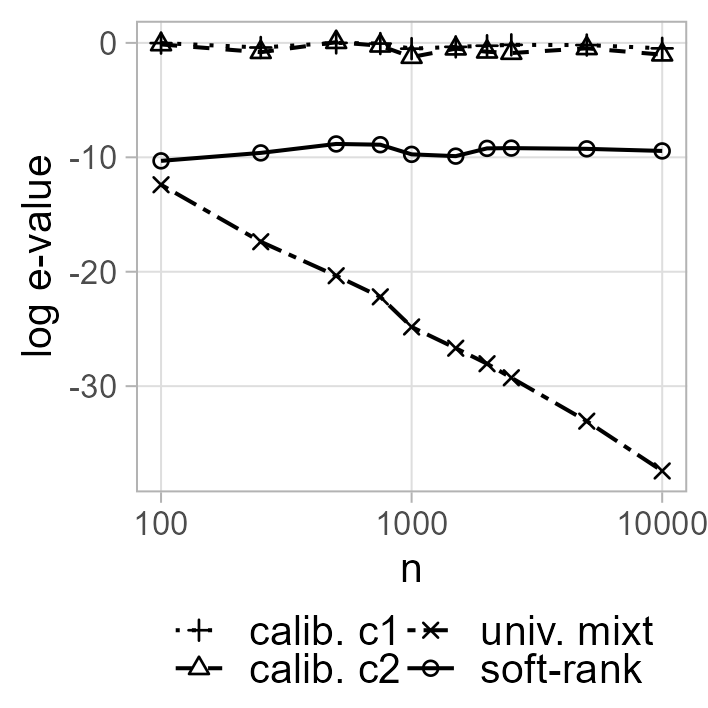
\includegraphics{images/sim.logreg.paper.beta0.png}  & 
         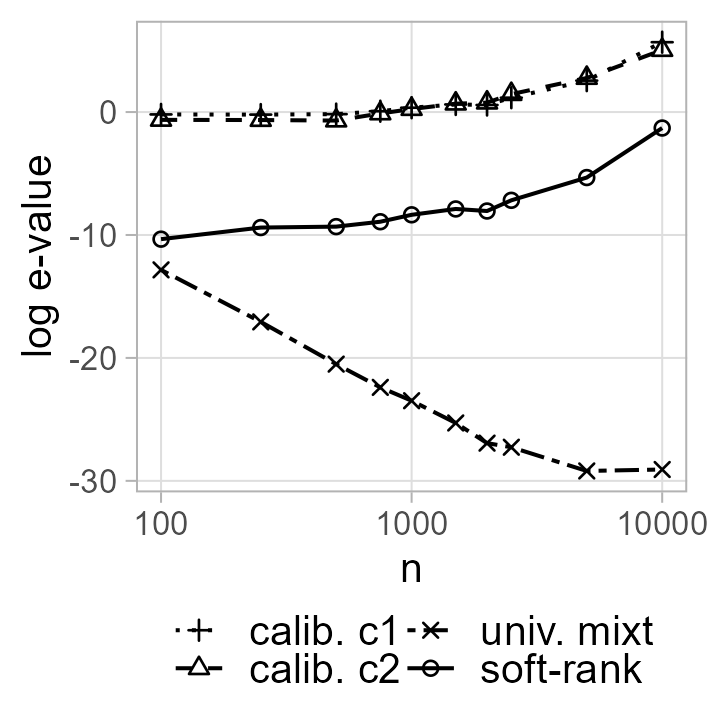
\includegraphics{images/sim.logreg.paper.beta0.15.png} \\
         $\beta_i^*=0.3$& $\beta_i^*=0.5$ \\
         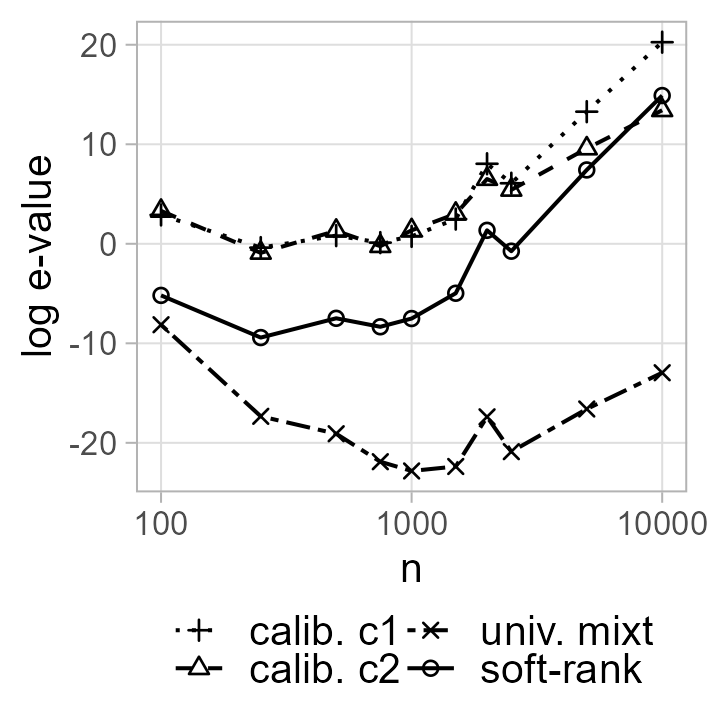
\includegraphics{images/sim.logreg.paper.beta0.3.png}  & 
         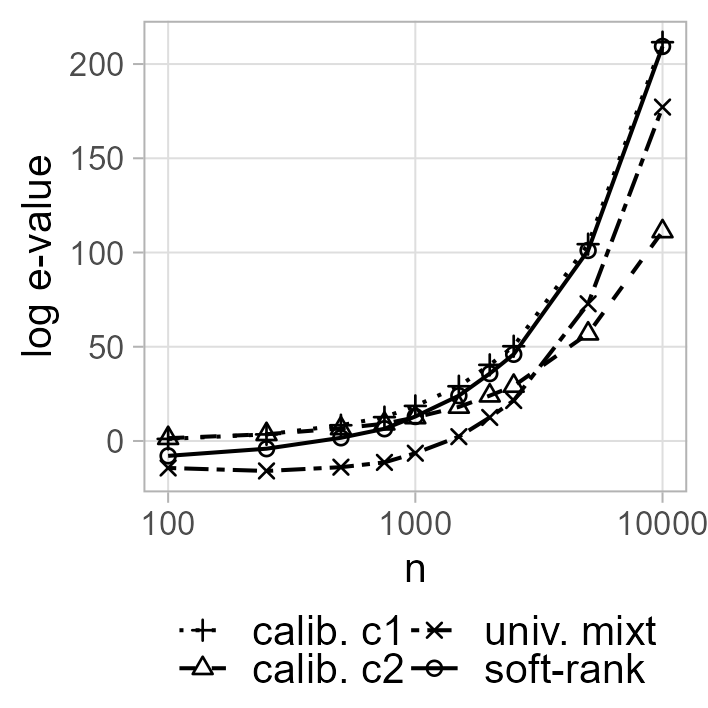
\includegraphics{images/sim.logreg.paper.beta0.5.png} \\
\end{tabular}
\caption{Average log e-values in logistic regression for $\beta_i^*=0$ (top left), $\beta_i^*=0.15$ (top right), $\beta_i^*=0.3$ (bottom left) and $\beta_i^*=0.5$ (bottom right) for universal mixture and soft-rank e-values, mixture (calib.c1) and inverse root p-to-e calibrators (calib.c2)}
\label{fig:simlogreg}
\end{figure}

\begin{table}[ht]
\caption{Empirical $P_{\beta^*_i=0} (E \geq 1/\alpha)$ (type I error) for $E\in\{E^{um},E^{sr},E^{c1},E^{c2}\}$ and $\alpha \in \{0.01,0.05\}$ in logistic regression}\label{tabtype1logreg}%
\begin{tabular}{ccc|cc|cc|cc}
\hline
n    & \multicolumn{2}{c|}{$E^{um}$} & \multicolumn{2}{c|}{$E^{sr}$}& \multicolumn{2}{c|}{$E^{c1}$} & \multicolumn{2}{c}{$E^{c2}$}\\ \hline
     & $\alpha=1\%$ & $\alpha=5\%$ & $\alpha=1\%$ & $\alpha=5\%$ & $\alpha=1\%$ & $\alpha=5\%$ & $\alpha=1\%$ & $\alpha=5\%$ \\
100  & 0                          & 0                          & 0                          & 0                          & 0                       & 0                       & 0.01                       & 0                      \\
500  & 0                          & 0                          & 0                          & 0                          & 0                          & 0                          & 0                          & 0                          \\
1500 & 0                          & 0                          & 0                          & 0                          & 0                          & 0                          & 0                          & 0                          \\
2000 & 0                          & 0                          & 0                          & 0                          & 0                          & 0                          & 0                          & 0                          \\ \hline
\end{tabular}
\end{table}


We assess the type I error control and power of the four strategies to obtain e-values discussed in Section \ref{ssec:define_evariables}: universal mixture and soft-rank e-values and the mixture and inverse root calibrators in \eqref{eq:calibrator1}-\eqref{eq:calibrator2}.
We run a simulation study in Gaussian linear and logistic regressions. We consider sample sizes $n$ ranging from 100 to 10,000 and 10 covariates. The covariates were generated from a zero-mean multivariate Gaussian with pairwise covariance $0.5$. Covariates were scaled to unit sample variance. For each family and each sample size, we simulate 100 datasets with data-generating regression coefficients $\beta_i^*\in[0,1]$, $i=1,\ldots,10$.

\david{If there are 0 type I errors for all methods and $n$ then no need to show the table, we can just say in the text that the there were no type I errors, to save space.}
\david{Here and in the table caption I'd say ``proportion of type I errors'' instead of ``empirical probability''. Question: how is it possible that $E^{c2}$ rejects more null hypotheses at the $\alpha=0.01$ than at the 0.05 level? If the simulations are run on the same datasets (which would give more precise estimates when comparing methods) then this cannot possibly occur.}
Table~\ref{tabtype1logreg} reports the empirical probability of type I error over the 100 repetitions for selected sample sizes in logistic regression. All considered e-variables exhibit good type I error control with empirical probabilities smaller or equal to the desired level. Figure~\ref{fig:simlogreg} plots the average log e-values over the 100 repetitions for $\beta_i^*\in \{0, 0.15, 0.3, 0.5\}$ in logistic regression. For nonzero $\beta_i^*$ and small $n$, the calibrated e-values $E^{c1}$ and $E^{c2}$ clearly dominate the universal mixture and soft-rank e-variables $E^{um}$ and $E^{sr}$, accumulating stronger evidence in favor of the alternative. For large $n$, the calibrated e-variable $E^{c2}$ became less competitive whereas the soft-rank e-variable $E^{sr}$ became more competitive, nearly matching the mixture calibrated e-variable $E^{c1}$ in some scenarios. 


\begin{table}[ht]
\caption{Empirical $P_{\beta^*_i=0} (E \geq 1/\alpha)$ (type I error) for $E\in\{E^{um},E^{sr},E^{c1},E^{c2}\}$ and $\alpha \in \{0.01,0.05\}$ in linear regression}\label{tabtype1linreg}%
\begin{tabular}{ccc|cc|cc|cc}
\hline
n    & \multicolumn{2}{c|}{$E^{um}$} & \multicolumn{2}{c|}{$E^{sr}$}& \multicolumn{2}{c|}{$E^{c1}$} & \multicolumn{2}{c}{$E^{c2}$}\\ \hline
     & $\alpha=1\%$ & $\alpha=5\%$ & $\alpha=1\%$ & $\alpha=5\%$ & $\alpha=1\%$ & $\alpha=5\%$ & $\alpha=1\%$ & $\alpha=5\%$ \\
100  & 0                          & 0                          & 0                          & 0                          & 0                       & 0                       & 0                       & 0                       \\
500  & 0                          & 0                          & 0                          & 0                          & 0                          & 0                          & 0                          & 0                          \\
1500 & 0                          & 0                          & 0                          & 0                          & 0                          & 0                          & 0                          & 0                          \\
2000 & 0                          & 0                          & 0                          & 0                          & 0                          & 0                          & 0                          & 0                          \\ \hline
\end{tabular}
\end{table}

\begin{figure}[ht]
\begin{tabular}{cc}
         $\beta_i^*=0$& $\beta_i^*=0.15$ \\
         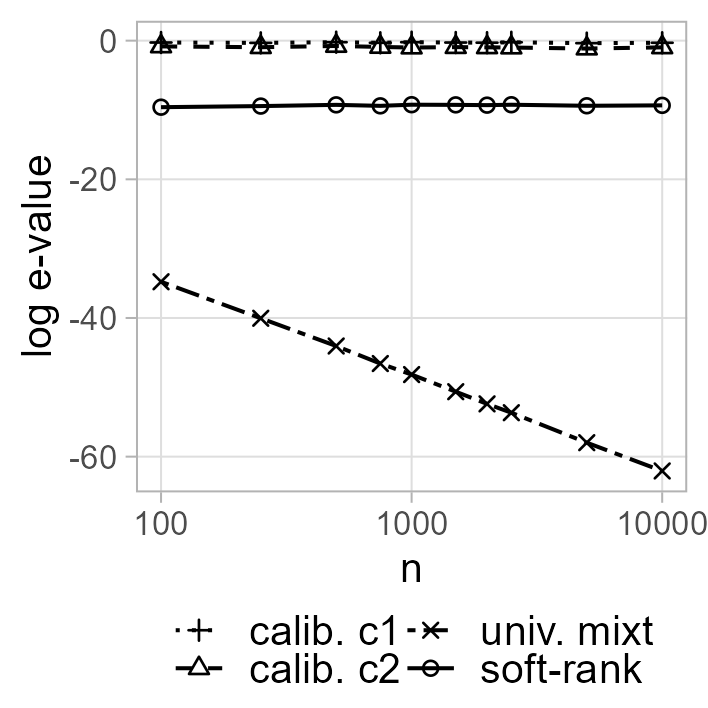
\includegraphics{images/sim.linreg.paper.beta0.png}  & 
         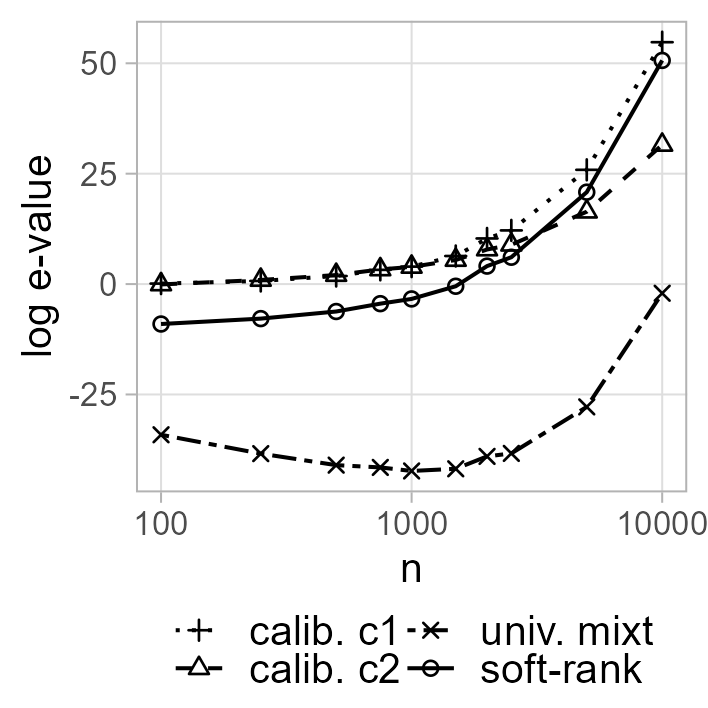
\includegraphics{images/sim.linreg.paper.beta0.15.png} \\
         $\beta_i^*=0.3$& $\beta_i^*=0.5$ \\
         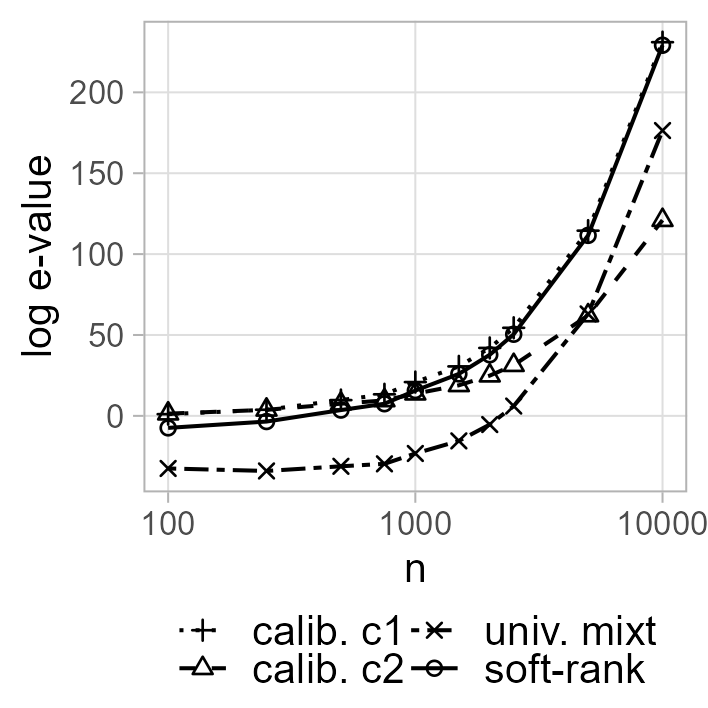
\includegraphics{images/sim.linreg.paper.beta0.3.png}  & 
         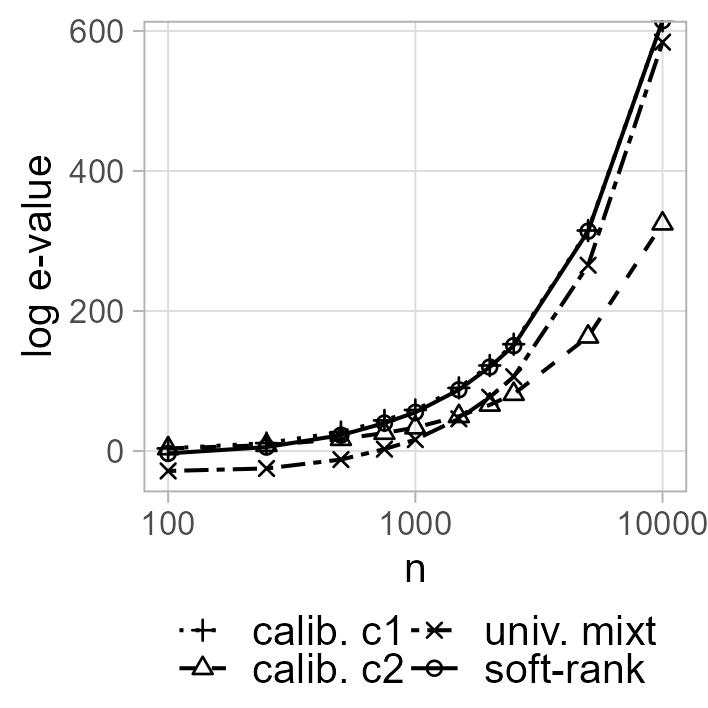
\includegraphics{images/sim.linreg.paper.beta0.5.png} \\
\end{tabular}
\caption{Average log e-values in linear regression for $\beta_i^*=0$ (top left), $\beta_i^*=0.15$ (top right), $\beta_i^*=0.3$ (bottom left) and $\beta_i^*=0.5$ (bottom right) for universal mixture and soft-rank e-values, mixture (calib.c1) and inverse root p-to-e calibrators (calib.c2)}
\label{fig:simlinreg}
\end{figure}


Table~\ref{tabtype1linreg} and Figure~\ref{fig:simlinreg} report, respectively, the empirical probability of type I error and the average log e-value for $\beta_i^*\in \{0, 0.15, 0.3, 0.5\}$ over the 100 repetitions in Gaussian linear regression. Findings are similar to that in logistic regression. In summary, out of the assessed e-variables, we recommend the mixture calibrator $E^{c1}$ to test the null hypotheses in \eqref{eq:test}, as it accrues stronger evidence for truly alternative hypotheses while appropriately controlling type I error. We remark that such e-values are only properly calibrated when the assumed model is correct (or approximately so), otherwise soft-rank e-variables may be preferable for being more robust to model misspecification.


\section{Results}
\label{sec:results}

\begin{figure}[ht]
\begin{tabular}{ccc}
         Depressed & Low self-esteem\\
         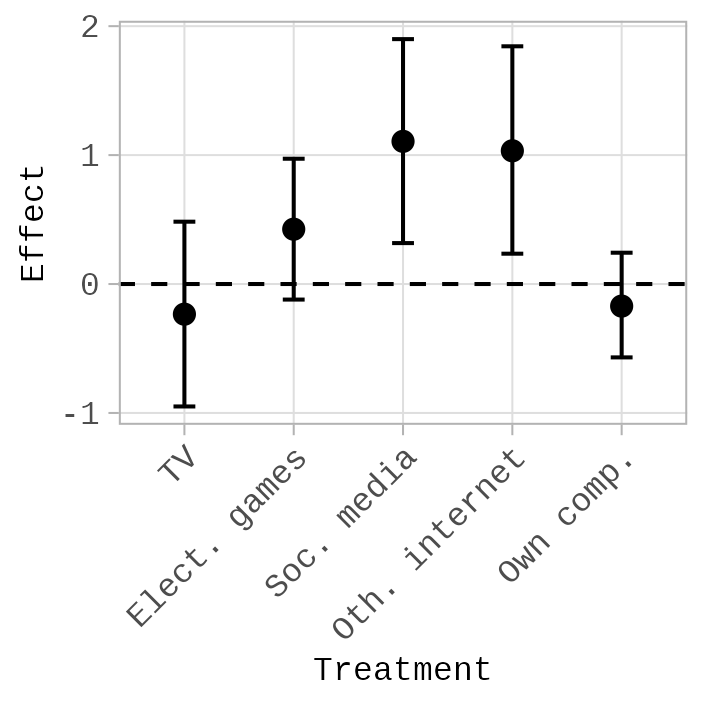
\includegraphics{images/plot.Ecidepressed.png}  & 
         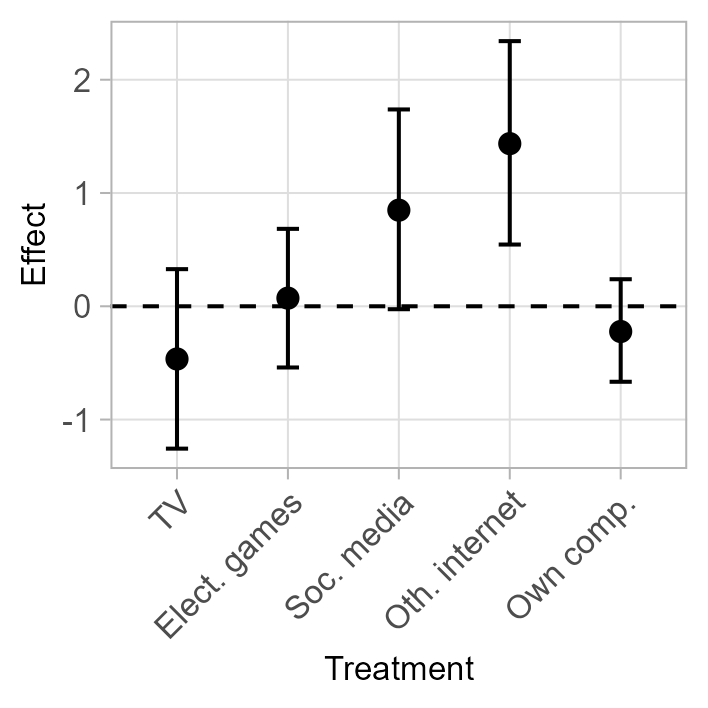
\includegraphics{images/plot.Eciselfesteem_lo.png} \\
         High total difficulties & High emotional problems\\
         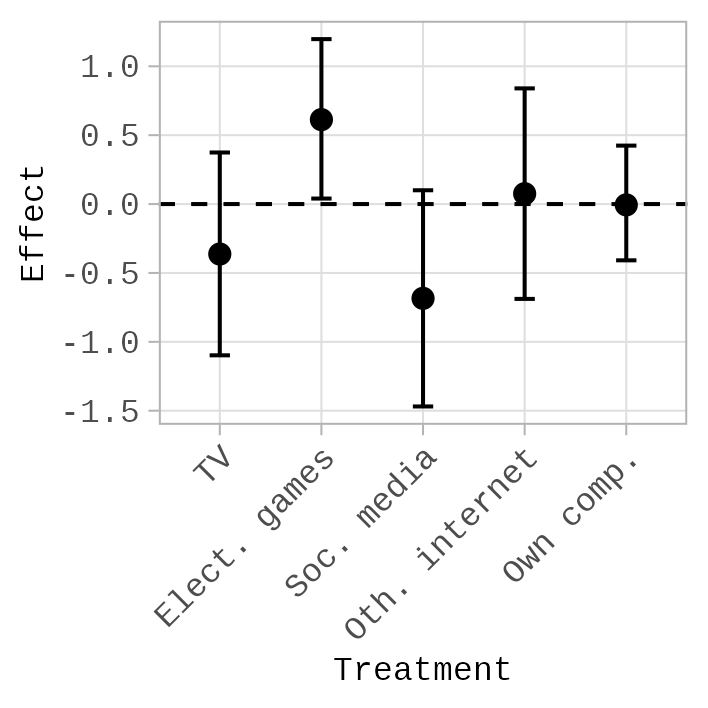
\includegraphics{images/plot.Ecifebdtot_hi.png}  & 
         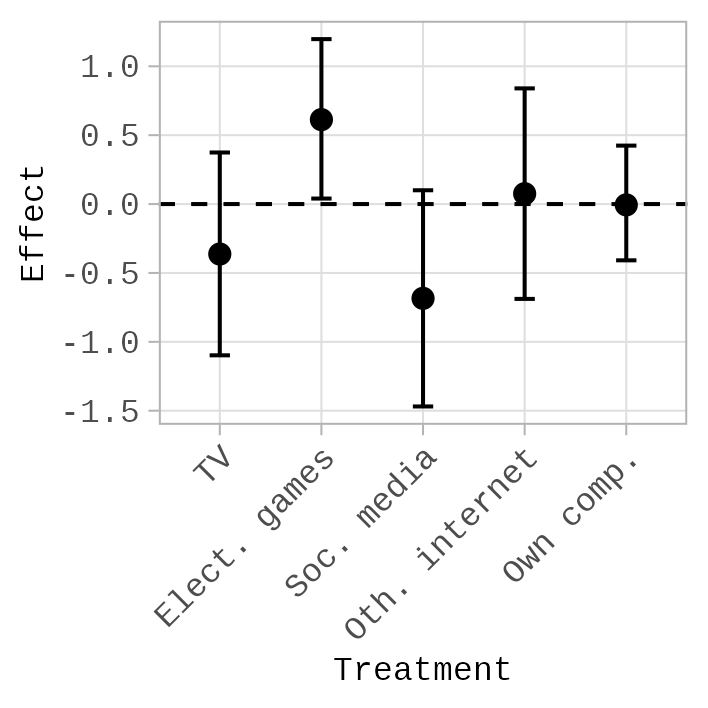
\includegraphics{images/plot.Ecifebdtot_hi.png} \\
         High conduct problems& High hyperactivity/inattention\\
         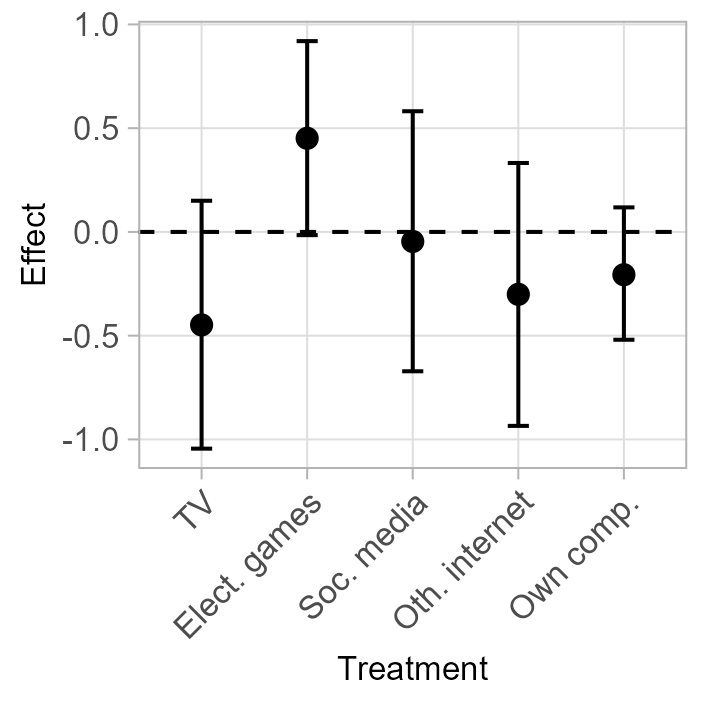
\includegraphics{images/plot.Ecifconduct_hi.png}  & 
         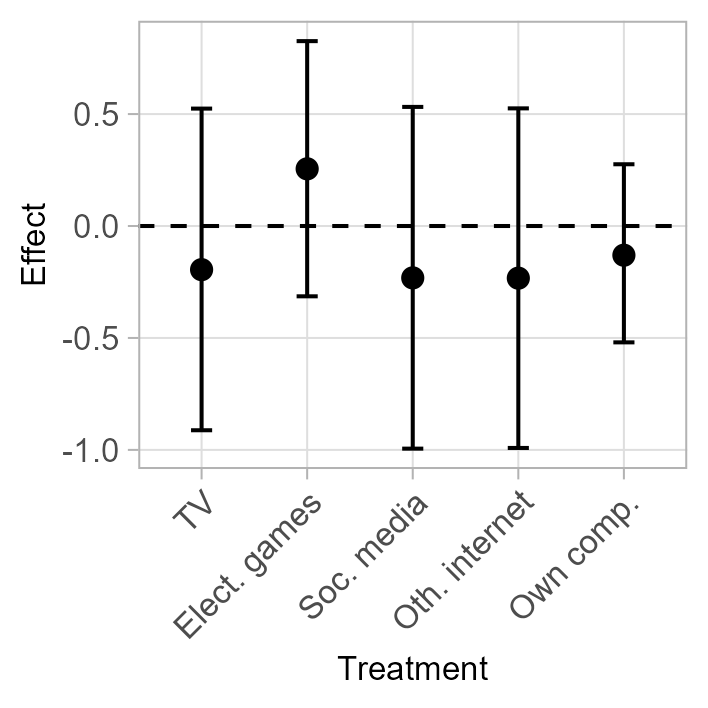
\includegraphics{images/plot.Ecifhyper_hi.png} \\
         High peer problems & Low pro-sociality\\
         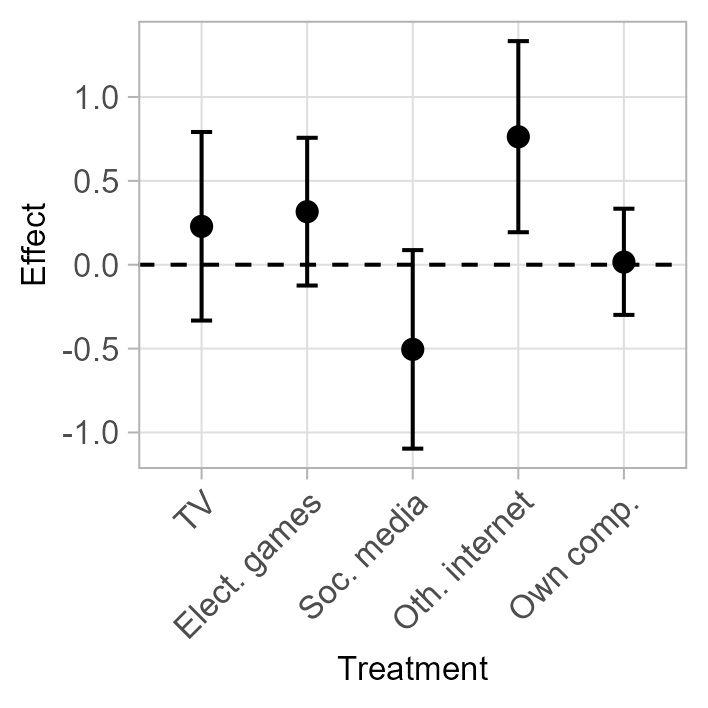
\includegraphics{images/plot.Ecifpeer_hi.png}  & 
         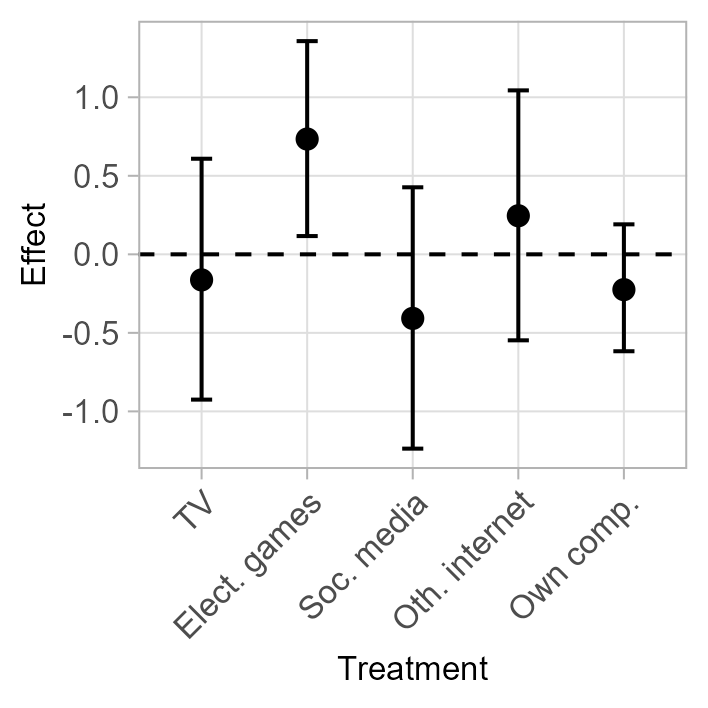
\includegraphics{images/plot.Ecifprosoc_lo.png}
        \end{tabular}
\caption{Estimated treatment effects by outcome under consideration and their corresponding 95\% c2-calibrated e-confidence interval.}
\label{fig:exp.mcs}
\end{figure}

\begin{table}[ht]
\caption{Rejected hypothesis by the refined eBH procedure with FDR level 0.05 using e-value $E^{c1}$, the corresponding estimated odds ratio, estimated effects and 95\% e-calibrated confidence intervals, and e-values.}\label{tab1}%
\begin{tabular}{@{}llcccc@{}}
\toprule
Outcome & Treatment & Odds ratio & Est. effect & 95\% conf. int. & e-value \\
\midrule
Low self-esteem   &  internet & 4.20 &  1.44 &(0.61,2.27) & 37,790 \\
Depressive symptoms    & social media & 3.02 & 1.11 &(0.38,1.85)  & 1,851\\
High peer problems & internet & 2.14  & 0.76 &(0.24,1.29)& 757 \\ 
Depressive symptoms &  internet & 2.81 & 1.03  &(0.29,1.78) & 396\\
\botrule
\end{tabular}
\end{table}

We apply our multiverse analysis framework to the study of the association between technology on teenager mental well-being in the 2015 survey of the Millennium Cohort Study (MCS). The MCS is a socio-economic and health survey tracking a representative sample of children born in the UK around year 2000 throughout their life. The 2015 data that we use has a rather large sample size, $n = 11,884$ teenagers, and features several outcome measures of mental well-being, $p_x=5$ treatments measuring the use of various technologies, and $p_z=14$ control covariates.

An earlier analysis of this dataset in~\cite{orben:2019} concluded that the association between technology and teenager well-being was not practically relevant. To assess significance of effects across outcomes and treatments, the authors used the Specification Curve Analysis~\cite{simonsohn:2020} method, which has serious shortcomings when used for proper statistical inference, as briefly discussed in Section~\ref{sec:intro}. When applied to MCS dataset, our framework leads to conclusions opposite to those in~\cite{orben:2019}.

We consider $L=8$ outcomes: self-assessed depressive symptoms (Mood and Feelings Questionnaire) and self-esteem (Rosenberg scale), as well as parent-assessed total difficulties, emotional problems, conduct problems, hyperactivity/inattention, peer problems and pro-sociality (all Strengths and Difficulties Questionnaire). There are $p_x=5$ treatments: time spent watching TV, playing video games, using the internet, using social media, and owning a personal computer. 
In all regressions, we include $p_z=14$ control covariates: gender, age, BMI, (self-reported) educational motivation, mother’s ethnicity, 
(self-reported) closeness to parents, presence of natural father, time spent with primary
caretaker (PC), PC’s word activity score, PC’s employment status, own longstanding
illness, PC’s psychological distress, number of siblings and household income.

The data were prepared as described in~\cite{semken:2022}. In particular, all treatment variables but TV usage were treated as
continuous variables, normalized such that 0 means “no usage” and 1 means maximum
reportable usage. TV usage was discretized into low, medium and high usage because its association with most outcomes was not linear (although it was monotone). The outcome variables are binary and were obtained by binning originally continuous data with validated cutoffs for abnormal behavior. See \cite{semken:2022} (Section S4) for further details on data pre-processing.

As an exploratory analysis, we plot in Figure~\ref{fig:exp.mcs} the mean treatment effects when fitting a logistic regression on each outcome against treatment and control variables. The reported 95\% confidence interval are e-confidence intervals~\cite{ramdas:2025} obtained by calibrating the standard profile confidence interval for logistic regression effects with calibrator $c2$ ($f(\pi)=\pi^{1/2}-1$). A total of 8 treatments appear significant. These intervals do not however account for the multiplicity and correlation of the hypotheses being tested.

Following our proposed framework, we compute next e-values for each outcome-treatment pair and apply the refined eBH procedure. In particular, we used the mixture calibrator e-variable $E^{c1}$ in \eqref{eq:calibrator1}, as it exhibited the largest power in our simulations. 
Before applying the eBH procedure, there were six hypotheses for which $1/E^{c1} > 20$, a thresholding which controls the individual type I error for each hypothesis at the 0.05 level.
Table~\ref{tab1} reports the subset of these that were rejected by the refined e-BH procedure, when controlling the FDR below 0.05. Alternative, less powerful, choices of e-variables in Section~\ref{ssec:define_evariables} (universal mixture, soft-rank and inverse root calibrator) lead to no rejection in this dataset after the refined eBH adjustment. Applying $\overline{\text{e-BH}}$ instead of the refined e-BH procedure did not alter any of the results. In total, four hypotheses are rejected by our framework suggesting a significant effect of technology on teenager well-being contrary to the original study in~\cite{orben:2019}. Specifically, a strong internet usage was found to be significantly associated with low self-steem and depressive symptoms as self-assessed by the teenagers, and high peer problems as assessed by their parents.
High social media usage was also found to be significantly associated with self-assessed depressive symptoms.
We remark that the odds-ratio for these associations were in the range $[2,4]$ \paul{is that large?} \david{they're certainly not negligible, it means that the odds of something bad happening are somewhere between 2 and 4 times higher. An OR of 1.5 is already relevant, typically.}, that is these findings are not only statistically significant but also practically relevant.
\david{In Table~\ref{tab1}, I guess that the confidence interval refers to the estimated coefficient not the OR correct? At first I thought that the CIs were for the OR which was then strange because they contain 0, which would mean they're not statistically significant. To avoid confusions, how about we just the OR and CI for the OR (i.e. exponentiate your current CI) and do not show the ``estimated effect'' -- it's a log-OR that's less easily interpretable anyway.}


%\section{Tables}\label{sec5}

%\begin{table}[h]
%\caption{Caption text}\label{tab1}%
%\begin{tabular}{@{}llll@{}}
%\toprule
%Column 1 & Column 2  & Column 3 & Column 4\\
%\midrule
%row 1    & data 1   & data 2  & data 3  \\
%row 2    & data 4   & data 5\footnotemark[1]  & data 6  \\
%row 3    & data 7   & data 8  & data 9\footnotemark[2]  \\
%\botrule
%\end{tabular}
%\footnotetext{Source: This is an example of table footnote. This is an example of table footnote.}
%\footnotetext[1]{Example for a first table footnote. This is an example of table footnote.}
%\footnotetext[2]{Example for a second table footnote. This is an example of table footnote.}
%\end{table}


%\begin{table}[h]
%\caption{Example of a lengthy table which is set to full textwidth}\label{tab2}
%\begin{tabular*}{\textwidth}{@{\extracolsep\fill}lcccccc}
%\toprule%
%& \multicolumn{3}{@{}c@{}}{Element 1\footnotemark[1]} & \multicolumn{3}{@{}c@{}}{Element 2\footnotemark[2]} \\\cmidrule{2-4}\cmidrule{5-7}%
%Project & Energy & $\sigma_{calc}$ & $\sigma_{expt}$ & Energy & $\sigma_{calc}$ & $\sigma_{expt}$ \\
%\midrule
%Element 3  & 990 A & 1168 & $1547\pm12$ & 780 A & 1166 & $1239\pm100$\\
%Element 4  & 500 A & 961  & $922\pm10$  & 900 A & 1268 & $1092\pm40$\\
%\botrule
%\end{tabular*}
%\footnotetext{Note: This is an example of table footnote. This is an example of table footnote this is an example of table footnote this is an example of~table footnote this is an example of table footnote.}
%\footnotetext[1]{Example for a first table footnote.}
%\footnotetext[2]{Example for a second table footnote.}
%\end{table}



\section{Discussion}
\label{sec:discussion}


Multiverse analysis is a useful tool to descriptively assess how the association between treatments and outcomes varies as one considers different treatments, outcomes, sub-populations of individuals, control covariates, or other analysis choices. When purely used in such a descriptive manner, it can help flag whether treatment-outcome associations are robust across analysis specifications or not.
A more contentious issue is when a multiverse analysis is used for formal statistical inference. In such situations, one must be careful to assess properly defined statistical estimands and to properly account for possible treatment effect heterogeneity. In particular, we do not recommend reporting averaged treatment effect estimates across all analysis specifications, except for fairly rare circumstances where the treatment and specifications are effectively viewed as exchangeable.
Instead, we recommend reporting treatment effects for all analysis specifications separately and accounting for the multiple comparisons being performed. This ensures statistical validity but has a cost in statistical power, which can be a practical issue when either the sample size of the treatment effect are relatively small.
For example, in the teenager data a previous analysis had found that the average effect across all treatments and outcomes was practically irrelevant, whereas assessing each treatment-outcome association separately reveals strong and very practically-relevant associations.

A further statistical issue is that many false positive control methods make strong assumptions about the hypotheses being performed (e.g., independence or positive dependence across hypotheses, many tests being performed, etc.). E-values may be an appealing FDR control strategy in this setting because they relax these assumptions, in particular they remain valid regardless of the dependence structure across the statistical tests and of the number of hypotheses tested. A concern however is that e-values can be conservative, in the sense of having low statistical power to detect treatment effects when they truly exist. Our simulations show that this issue is much more marked for some strategies than for others, and these findings were confirmed in the teenager mental well-being data. Mixture calibrated e-variables worked best in our experiments, whereas on the other end of the spectrum universal mixture e-variables were extremely conservative in our examples, to the point of being practically useless unless $n$ or the treatment effects are extremely large. Soft-rank e-variables were less powerful than mixture calibrated e-variables, particularly for small $n$, but they may be appealing in settings where the model is misspecified.

In conclusion, our results suggest that e-variables can be a useful complement to multiverse analyses, but they also point to significant limitations in terms of their statistical power. Hence, they should be viewed as a conservative procedure that is best suited for moderately large sample sizes and treatment effect sizes. We also remark that e-variables is a recent framework and that there is active research in designing more powerful e-variables, which may improve their properties when used within multiverse analyses.


\backmatter

%\bmhead{Supplementary information}
% 
%If your article has accompanying supplementary file/s please state so here. 
% 


\section*{Declarations}

\bmhead{Funding}

DR was funded by grant 0045 within the ICREA Academia program from AGAUR (Generalitat de Catalunya), and by grant PID2022-138268NB-I00 by Ministerio de Ciencia e Innovaci\'on (MICIN)/Agencia Espa\~{n}ola de Investigaci\'on(AEI)/10.13039/501100011033 /Fondo Europeo de Desarrollo Regional (FEDER). Co-funded by the European Union (ERC, BigBayesUQ, project number: 101041064). Views and opinions expressed are however those of the author(s) only and do not necessarily reflect those of the European Union or the European Research Council. Neither the European Union nor the granting authority can be held responsible for them.

\bmhead{Ethics approval}

Not applicable.

\bmhead{Consent}

Not applicable.

\bmhead{Data}

The code is available XXXX.

\bmhead{Code availability}

The code is available XXXX.

\bmhead{Author's contribution statements}

All authors contributed equally to this work.

%If any of the sections are not relevant to your manuscript, please include the heading and write `Not applicable' for that section. 


% \begin{appendices}

% \section{Section title of first appendix}\label{secA1}

%\end{appendices}


\bibliography{references}% common bib file
%% if required, the content of .bbl file can be included here once bbl is generated
%%\input sn-article.bbl

\end{document}
